\documentclass[twoside]{book}

% Packages required by doxygen
\usepackage{calc}
\usepackage{doxygen}
\usepackage{graphicx}
\usepackage[utf8]{inputenc}
\usepackage{makeidx}
\usepackage{multicol}
\usepackage{multirow}
\usepackage{textcomp}
\usepackage[table]{xcolor}

% Font selection
\usepackage[T1]{fontenc}
\usepackage{mathptmx}
\usepackage[scaled=.90]{helvet}
\usepackage{courier}
\usepackage{amssymb}
\usepackage{sectsty}
\renewcommand{\familydefault}{\sfdefault}
\allsectionsfont{%
  \fontseries{bc}\selectfont%
  \color{darkgray}%
}
\renewcommand{\DoxyLabelFont}{%
  \fontseries{bc}\selectfont%
  \color{darkgray}%
}

% Page & text layout
\usepackage{geometry}
\geometry{%
  a4paper,%
  top=2.5cm,%
  bottom=2.5cm,%
  left=2.5cm,%
  right=2.5cm%
}
\tolerance=750
\hfuzz=15pt
\hbadness=750
\setlength{\emergencystretch}{15pt}
\setlength{\parindent}{0cm}
\setlength{\parskip}{0.2cm}
\makeatletter
\renewcommand{\paragraph}{%
  \@startsection{paragraph}{4}{0ex}{-1.0ex}{1.0ex}{%
    \normalfont\normalsize\bfseries\SS@parafont%
  }%
}
\renewcommand{\subparagraph}{%
  \@startsection{subparagraph}{5}{0ex}{-1.0ex}{1.0ex}{%
    \normalfont\normalsize\bfseries\SS@subparafont%
  }%
}
\makeatother

% Headers & footers
\usepackage{fancyhdr}
\pagestyle{fancyplain}
\fancyhead[LE]{\fancyplain{}{\bfseries\thepage}}
\fancyhead[CE]{\fancyplain{}{}}
\fancyhead[RE]{\fancyplain{}{\bfseries\leftmark}}
\fancyhead[LO]{\fancyplain{}{\bfseries\rightmark}}
\fancyhead[CO]{\fancyplain{}{}}
\fancyhead[RO]{\fancyplain{}{\bfseries\thepage}}
\fancyfoot[LE]{\fancyplain{}{}}
\fancyfoot[CE]{\fancyplain{}{}}
\fancyfoot[RE]{\fancyplain{}{\bfseries\scriptsize Generated on Mon May 9 2016 15\-:35\-:19 for My Project by Doxygen }}
\fancyfoot[LO]{\fancyplain{}{\bfseries\scriptsize Generated on Mon May 9 2016 15\-:35\-:19 for My Project by Doxygen }}
\fancyfoot[CO]{\fancyplain{}{}}
\fancyfoot[RO]{\fancyplain{}{}}
\renewcommand{\footrulewidth}{0.4pt}
\renewcommand{\chaptermark}[1]{%
  \markboth{#1}{}%
}
\renewcommand{\sectionmark}[1]{%
  \markright{\thesection\ #1}%
}

% Indices & bibliography
\usepackage{natbib}
\usepackage[titles]{tocloft}
\setcounter{tocdepth}{3}
\setcounter{secnumdepth}{5}
\makeindex

% Hyperlinks (required, but should be loaded last)
\usepackage{ifpdf}
\ifpdf
  \usepackage[pdftex,pagebackref=true]{hyperref}
\else
  \usepackage[ps2pdf,pagebackref=true]{hyperref}
\fi
\hypersetup{%
  colorlinks=true,%
  linkcolor=blue,%
  citecolor=blue,%
  unicode%
}

% Custom commands
\newcommand{\clearemptydoublepage}{%
  \newpage{\pagestyle{empty}\cleardoublepage}%
}


%===== C O N T E N T S =====

\begin{document}

% Titlepage & ToC
\hypersetup{pageanchor=false}
\pagenumbering{roman}
\begin{titlepage}
\vspace*{7cm}
\begin{center}%
{\Large My Project }\\
\vspace*{1cm}
{\large Generated by Doxygen 1.8.6}\\
\vspace*{0.5cm}
{\small Mon May 9 2016 15:35:19}\\
\end{center}
\end{titlepage}
\clearemptydoublepage
\tableofcontents
\clearemptydoublepage
\pagenumbering{arabic}
\hypersetup{pageanchor=true}

%--- Begin generated contents ---
\chapter{Hierarchical Index}
\section{Class Hierarchy}
This inheritance list is sorted roughly, but not completely, alphabetically\-:\begin{DoxyCompactList}
\item \contentsline{section}{Basic\-Tabu\-Search}{\pageref{classBasicTabuSearch}}{}
\item \contentsline{section}{Binary\-Search}{\pageref{classBinarySearch}}{}
\item \contentsline{section}{Coloration}{\pageref{classColoration}}{}
\item \contentsline{section}{Graphe}{\pageref{classGraphe}}{}
\item \contentsline{section}{Iterated\-Tabu\-Search}{\pageref{classIteratedTabuSearch}}{}
\item \contentsline{section}{Voisin}{\pageref{classVoisin}}{}
\begin{DoxyCompactList}
\item \contentsline{section}{One\-Move}{\pageref{classOneMove}}{}
\item \contentsline{section}{Swap}{\pageref{classSwap}}{}
\end{DoxyCompactList}
\end{DoxyCompactList}

\chapter{Class Index}
\section{Class List}
Here are the classes, structs, unions and interfaces with brief descriptions\-:\begin{DoxyCompactList}
\item\contentsline{section}{\hyperlink{classBasicTabuSearch}{Basic\-Tabu\-Search} }{\pageref{classBasicTabuSearch}}{}
\item\contentsline{section}{\hyperlink{classBinarySearch}{Binary\-Search} }{\pageref{classBinarySearch}}{}
\item\contentsline{section}{\hyperlink{classColoration}{Coloration} }{\pageref{classColoration}}{}
\item\contentsline{section}{\hyperlink{classGraphe}{Graphe} }{\pageref{classGraphe}}{}
\item\contentsline{section}{\hyperlink{classIteratedTabuSearch}{Iterated\-Tabu\-Search} }{\pageref{classIteratedTabuSearch}}{}
\item\contentsline{section}{\hyperlink{classOneMove}{One\-Move} }{\pageref{classOneMove}}{}
\item\contentsline{section}{\hyperlink{classSwap}{Swap} }{\pageref{classSwap}}{}
\item\contentsline{section}{\hyperlink{classVoisin}{Voisin} }{\pageref{classVoisin}}{}
\end{DoxyCompactList}

\chapter{Class Documentation}
\hypertarget{classBasicTabuSearch}{\section{Basic\-Tabu\-Search Class Reference}
\label{classBasicTabuSearch}\index{Basic\-Tabu\-Search@{Basic\-Tabu\-Search}}
}


{\ttfamily \#include $<$basictabusearch.\-h$>$}

\subsection*{Public Member Functions}
\begin{DoxyCompactItemize}
\item 
\hyperlink{classBasicTabuSearch_a30a404fa4c0c95bdbfdf9b8d9387145b}{Basic\-Tabu\-Search} (\hyperlink{classColoration}{Coloration} $\ast$init, int prof)
\item 
\hyperlink{classBasicTabuSearch_ad4449024a20e6609dd20884696356c8a}{$\sim$\-Basic\-Tabu\-Search} ()
\item 
\hyperlink{classColoration}{Coloration} $\ast$ \hyperlink{classBasicTabuSearch_a439b45b01e2fb3c39668deaabdce6945}{run} ()
\item 
void \hyperlink{classBasicTabuSearch_ae51343045059a6e810b962429b8928d6}{init\-Tabu\-Mat} ()
\item 
void \hyperlink{classBasicTabuSearch_aa64a2c376b8e8c594163c1967126bb15}{init\-Neighboor\-O\-M} ()
\item 
void \hyperlink{classBasicTabuSearch_ae84e184edf1ef484d53107759433613b}{init\-Neighboor\-S} ()
\item 
void \hyperlink{classBasicTabuSearch_a14a157e898bba846f3b00f25b7c64fe2}{calcul\-Delta} ()
\item 
bool \hyperlink{classBasicTabuSearch_aa88417b74f0d99d694309226306eedef}{is\-Forbidden} (\hyperlink{classVoisin}{Voisin} $\ast$N, int iter)
\item 
bool \hyperlink{classBasicTabuSearch_af4f4afee741e09940ea4b8c47468613a}{is\-Forbidden\-O\-M} (\hyperlink{classOneMove}{One\-Move} $\ast$om, int iter)
\item 
bool \hyperlink{classBasicTabuSearch_a6d5c0de432bfe36a379e0cdb52457728}{is\-Forbidden\-S} (\hyperlink{classSwap}{Swap} $\ast$s, int iter)
\end{DoxyCompactItemize}


\subsection{Detailed Description}
Cette classe représente la procédure de recherche Tabou initiale présentée au point 2.\-4.\-2 de l'article lié. Le coeur de cette classe est le méthode \hyperlink{classBasicTabuSearch_a439b45b01e2fb3c39668deaabdce6945}{run()} éxecutant la recherche selon les paramètres de l'instance et retournant un pointeur sur la meilleure coloration trouvée. 

\subsection{Constructor \& Destructor Documentation}
\hypertarget{classBasicTabuSearch_a30a404fa4c0c95bdbfdf9b8d9387145b}{\index{Basic\-Tabu\-Search@{Basic\-Tabu\-Search}!Basic\-Tabu\-Search@{Basic\-Tabu\-Search}}
\index{Basic\-Tabu\-Search@{Basic\-Tabu\-Search}!BasicTabuSearch@{Basic\-Tabu\-Search}}
\subsubsection[{Basic\-Tabu\-Search}]{\setlength{\rightskip}{0pt plus 5cm}Basic\-Tabu\-Search\-::\-Basic\-Tabu\-Search (
\begin{DoxyParamCaption}
\item[{{\bf Coloration} $\ast$}]{init, }
\item[{int}]{prof}
\end{DoxyParamCaption}
)}}\label{classBasicTabuSearch_a30a404fa4c0c95bdbfdf9b8d9387145b}
Constructeur unique 
\begin{DoxyParams}{Parameters}
{\em init} & \hyperlink{classColoration}{Coloration} initiale de la recherche tabou \\
\hline
{\em prof} & profondeur de la recherche tabou \\
\hline
\end{DoxyParams}
\hypertarget{classBasicTabuSearch_ad4449024a20e6609dd20884696356c8a}{\index{Basic\-Tabu\-Search@{Basic\-Tabu\-Search}!$\sim$\-Basic\-Tabu\-Search@{$\sim$\-Basic\-Tabu\-Search}}
\index{$\sim$\-Basic\-Tabu\-Search@{$\sim$\-Basic\-Tabu\-Search}!BasicTabuSearch@{Basic\-Tabu\-Search}}
\subsubsection[{$\sim$\-Basic\-Tabu\-Search}]{\setlength{\rightskip}{0pt plus 5cm}Basic\-Tabu\-Search\-::$\sim$\-Basic\-Tabu\-Search (
\begin{DoxyParamCaption}
{}
\end{DoxyParamCaption}
)}}\label{classBasicTabuSearch_ad4449024a20e6609dd20884696356c8a}
Destructeur 

\subsection{Member Function Documentation}
\hypertarget{classBasicTabuSearch_a14a157e898bba846f3b00f25b7c64fe2}{\index{Basic\-Tabu\-Search@{Basic\-Tabu\-Search}!calcul\-Delta@{calcul\-Delta}}
\index{calcul\-Delta@{calcul\-Delta}!BasicTabuSearch@{Basic\-Tabu\-Search}}
\subsubsection[{calcul\-Delta}]{\setlength{\rightskip}{0pt plus 5cm}void Basic\-Tabu\-Search\-::calcul\-Delta (
\begin{DoxyParamCaption}
{}
\end{DoxyParamCaption}
)}}\label{classBasicTabuSearch_a14a157e898bba846f3b00f25b7c64fe2}
Fonction calculant le gain associé à l'ensemble des voisins admissibles \hypertarget{classBasicTabuSearch_aa64a2c376b8e8c594163c1967126bb15}{\index{Basic\-Tabu\-Search@{Basic\-Tabu\-Search}!init\-Neighboor\-O\-M@{init\-Neighboor\-O\-M}}
\index{init\-Neighboor\-O\-M@{init\-Neighboor\-O\-M}!BasicTabuSearch@{Basic\-Tabu\-Search}}
\subsubsection[{init\-Neighboor\-O\-M}]{\setlength{\rightskip}{0pt plus 5cm}void Basic\-Tabu\-Search\-::init\-Neighboor\-O\-M (
\begin{DoxyParamCaption}
{}
\end{DoxyParamCaption}
)}}\label{classBasicTabuSearch_aa64a2c376b8e8c594163c1967126bb15}
Fonction calculant l'ensemble des voisins \hyperlink{classOneMove}{One\-Move} admissibles par la solution courante. \hypertarget{classBasicTabuSearch_ae84e184edf1ef484d53107759433613b}{\index{Basic\-Tabu\-Search@{Basic\-Tabu\-Search}!init\-Neighboor\-S@{init\-Neighboor\-S}}
\index{init\-Neighboor\-S@{init\-Neighboor\-S}!BasicTabuSearch@{Basic\-Tabu\-Search}}
\subsubsection[{init\-Neighboor\-S}]{\setlength{\rightskip}{0pt plus 5cm}void Basic\-Tabu\-Search\-::init\-Neighboor\-S (
\begin{DoxyParamCaption}
{}
\end{DoxyParamCaption}
)}}\label{classBasicTabuSearch_ae84e184edf1ef484d53107759433613b}
Fonction calculant l'ensemble des voisins \hyperlink{classSwap}{Swap} admissibles par la solution courante. \hypertarget{classBasicTabuSearch_ae51343045059a6e810b962429b8928d6}{\index{Basic\-Tabu\-Search@{Basic\-Tabu\-Search}!init\-Tabu\-Mat@{init\-Tabu\-Mat}}
\index{init\-Tabu\-Mat@{init\-Tabu\-Mat}!BasicTabuSearch@{Basic\-Tabu\-Search}}
\subsubsection[{init\-Tabu\-Mat}]{\setlength{\rightskip}{0pt plus 5cm}void Basic\-Tabu\-Search\-::init\-Tabu\-Mat (
\begin{DoxyParamCaption}
{}
\end{DoxyParamCaption}
)}}\label{classBasicTabuSearch_ae51343045059a6e810b962429b8928d6}
Fonction d'initalisation de la matrice tabou. \hypertarget{classBasicTabuSearch_aa88417b74f0d99d694309226306eedef}{\index{Basic\-Tabu\-Search@{Basic\-Tabu\-Search}!is\-Forbidden@{is\-Forbidden}}
\index{is\-Forbidden@{is\-Forbidden}!BasicTabuSearch@{Basic\-Tabu\-Search}}
\subsubsection[{is\-Forbidden}]{\setlength{\rightskip}{0pt plus 5cm}bool Basic\-Tabu\-Search\-::is\-Forbidden (
\begin{DoxyParamCaption}
\item[{{\bf Voisin} $\ast$}]{N, }
\item[{int}]{iter}
\end{DoxyParamCaption}
)}}\label{classBasicTabuSearch_aa88417b74f0d99d694309226306eedef}
Procédure de vérification qu'un mouvement de voisinage n'est pas interdit Effectue un dynamic\-\_\-cast et appelle la fonction correspondante 
\begin{DoxyParams}{Parameters}
{\em N} & \hyperlink{classVoisin}{Voisin} à caster et tester \\
\hline
{\em iter} & iteration courante \\
\hline
\end{DoxyParams}
\begin{DoxyReturn}{Returns}
resultat de la sous-\/fonction appelée 
\end{DoxyReturn}
\hypertarget{classBasicTabuSearch_af4f4afee741e09940ea4b8c47468613a}{\index{Basic\-Tabu\-Search@{Basic\-Tabu\-Search}!is\-Forbidden\-O\-M@{is\-Forbidden\-O\-M}}
\index{is\-Forbidden\-O\-M@{is\-Forbidden\-O\-M}!BasicTabuSearch@{Basic\-Tabu\-Search}}
\subsubsection[{is\-Forbidden\-O\-M}]{\setlength{\rightskip}{0pt plus 5cm}bool Basic\-Tabu\-Search\-::is\-Forbidden\-O\-M (
\begin{DoxyParamCaption}
\item[{{\bf One\-Move} $\ast$}]{om, }
\item[{int}]{iter}
\end{DoxyParamCaption}
)}}\label{classBasicTabuSearch_af4f4afee741e09940ea4b8c47468613a}
Procédure de vérification qu'un \hyperlink{classOneMove}{One\-Move} ne soit pas interdit 
\begin{DoxyParams}{Parameters}
{\em om} & \hyperlink{classOneMove}{One\-Move} à tester \\
\hline
{\em iter} & iteration courante de la recherche \\
\hline
\end{DoxyParams}
\begin{DoxyReturn}{Returns}
( tabu\-Mat\mbox{[}om-\/$>$get\-S()\mbox{]}\mbox{[}om-\/$>$get\-Vkj()\mbox{]} $>$ iter ) 
\end{DoxyReturn}
\hypertarget{classBasicTabuSearch_a6d5c0de432bfe36a379e0cdb52457728}{\index{Basic\-Tabu\-Search@{Basic\-Tabu\-Search}!is\-Forbidden\-S@{is\-Forbidden\-S}}
\index{is\-Forbidden\-S@{is\-Forbidden\-S}!BasicTabuSearch@{Basic\-Tabu\-Search}}
\subsubsection[{is\-Forbidden\-S}]{\setlength{\rightskip}{0pt plus 5cm}bool Basic\-Tabu\-Search\-::is\-Forbidden\-S (
\begin{DoxyParamCaption}
\item[{{\bf Swap} $\ast$}]{s, }
\item[{int}]{iter}
\end{DoxyParamCaption}
)}}\label{classBasicTabuSearch_a6d5c0de432bfe36a379e0cdb52457728}
Procédure de vérification qu'un \hyperlink{classSwap}{Swap} ne soit pas interdit 
\begin{DoxyParams}{Parameters}
{\em s} & \hyperlink{classSwap}{Swap} à tester \\
\hline
{\em iter} & iteration courante de la recherche \\
\hline
\end{DoxyParams}
\begin{DoxyReturn}{Returns}
( (tabu\-Mat\mbox{[}s-\/$>$get\-Si()\mbox{]}\mbox{[}s-\/$>$get\-Kj()\mbox{]} $>$ iter) $\vert$$\vert$ (tabu\-Mat\mbox{[}s-\/$>$get\-Sj()\mbox{]}\mbox{[}s-\/$>$get\-Ki()\mbox{]} $>$ iter) ) 
\end{DoxyReturn}
\hypertarget{classBasicTabuSearch_a439b45b01e2fb3c39668deaabdce6945}{\index{Basic\-Tabu\-Search@{Basic\-Tabu\-Search}!run@{run}}
\index{run@{run}!BasicTabuSearch@{Basic\-Tabu\-Search}}
\subsubsection[{run}]{\setlength{\rightskip}{0pt plus 5cm}{\bf Coloration} $\ast$ Basic\-Tabu\-Search\-::run (
\begin{DoxyParamCaption}
{}
\end{DoxyParamCaption}
)}}\label{classBasicTabuSearch_a439b45b01e2fb3c39668deaabdce6945}
Méthode principale de la recherche tabou basique Respecte l'algorithme décrit au point 2.\-4.\-2 de l'article lié. \begin{DoxyReturn}{Returns}
meilleur coloration trouvée. 
\end{DoxyReturn}


The documentation for this class was generated from the following files\-:\begin{DoxyCompactItemize}
\item 
basictabusearch.\-h\item 
basictabusearch.\-cpp\end{DoxyCompactItemize}

\hypertarget{classBinarySearch}{\section{Binary\-Search Class Reference}
\label{classBinarySearch}\index{Binary\-Search@{Binary\-Search}}
}


{\ttfamily \#include $<$binarysearch.\-h$>$}

\subsection*{Public Member Functions}
\begin{DoxyCompactItemize}
\item 
\hyperlink{classBinarySearch_a189641a6509564e762d4910efa5ff234}{Binary\-Search} (\hyperlink{classGraphe}{Graphe} $\ast$graphe, int d)
\item 
\hyperlink{classBinarySearch_a580de16a971e9cc0721bfe4ad438034e}{Binary\-Search} (const \hyperlink{classBinarySearch}{Binary\-Search} \&other)
\item 
virtual \hyperlink{classBinarySearch_a2b99e8ebae410b1af5456456f806f86f}{$\sim$\-Binary\-Search} ()
\item 
\hyperlink{classColoration}{Coloration} $\ast$ \hyperlink{classBinarySearch_a8c4be01a34f8a443889466a77fa4c437}{run} ()
\end{DoxyCompactItemize}


\subsection{Detailed Description}
Cette classe représente la recherche binaire permettant dans le papier étudié de déterminer un nombre de couleur initial interessant pour ensuite effectuer une recherche tabou itérée.

Pour plus de détails, veuillez-\/vous reportez à la section 2.\-3 de l'article de référence \-:

\href{http://www.info.univ-angers.fr/pub/hao/papers/LaiHaoGloverEAAI2015.pdf}{\tt http\-://www.\-info.\-univ-\/angers.\-fr/pub/hao/papers/\-Lai\-Hao\-Glover\-E\-A\-A\-I2015.\-pdf} $\ast$ 

\subsection{Constructor \& Destructor Documentation}
\hypertarget{classBinarySearch_a189641a6509564e762d4910efa5ff234}{\index{Binary\-Search@{Binary\-Search}!Binary\-Search@{Binary\-Search}}
\index{Binary\-Search@{Binary\-Search}!BinarySearch@{Binary\-Search}}
\subsubsection[{Binary\-Search}]{\setlength{\rightskip}{0pt plus 5cm}Binary\-Search\-::\-Binary\-Search (
\begin{DoxyParamCaption}
\item[{{\bf Graphe} $\ast$}]{graphe, }
\item[{int}]{d}
\end{DoxyParamCaption}
)}}\label{classBinarySearch_a189641a6509564e762d4910efa5ff234}
Constructeur par défaut. 
\begin{DoxyParams}{Parameters}
{\em graphe} & \hyperlink{classGraphe}{Graphe} concerné par l'étude de l'E\-C\-P en cours \\
\hline
{\em d} & profondeur de la \hyperlink{classBasicTabuSearch}{Basic\-Tabu\-Search} utilisée au cours de l'execution \\
\hline
\end{DoxyParams}
\hypertarget{classBinarySearch_a580de16a971e9cc0721bfe4ad438034e}{\index{Binary\-Search@{Binary\-Search}!Binary\-Search@{Binary\-Search}}
\index{Binary\-Search@{Binary\-Search}!BinarySearch@{Binary\-Search}}
\subsubsection[{Binary\-Search}]{\setlength{\rightskip}{0pt plus 5cm}Binary\-Search\-::\-Binary\-Search (
\begin{DoxyParamCaption}
\item[{const {\bf Binary\-Search} \&}]{other}
\end{DoxyParamCaption}
)}}\label{classBinarySearch_a580de16a971e9cc0721bfe4ad438034e}
Constructeur par recopie 
\begin{DoxyParams}{Parameters}
{\em other} & référence sur la copie servant d'initialiseur \\
\hline
\end{DoxyParams}
\hypertarget{classBinarySearch_a2b99e8ebae410b1af5456456f806f86f}{\index{Binary\-Search@{Binary\-Search}!$\sim$\-Binary\-Search@{$\sim$\-Binary\-Search}}
\index{$\sim$\-Binary\-Search@{$\sim$\-Binary\-Search}!BinarySearch@{Binary\-Search}}
\subsubsection[{$\sim$\-Binary\-Search}]{\setlength{\rightskip}{0pt plus 5cm}Binary\-Search\-::$\sim$\-Binary\-Search (
\begin{DoxyParamCaption}
{}
\end{DoxyParamCaption}
)\hspace{0.3cm}{\ttfamily [virtual]}}}\label{classBinarySearch_a2b99e8ebae410b1af5456456f806f86f}
Destructeur 

\subsection{Member Function Documentation}
\hypertarget{classBinarySearch_a8c4be01a34f8a443889466a77fa4c437}{\index{Binary\-Search@{Binary\-Search}!run@{run}}
\index{run@{run}!BinarySearch@{Binary\-Search}}
\subsubsection[{run}]{\setlength{\rightskip}{0pt plus 5cm}{\bf Coloration} $\ast$ Binary\-Search\-::run (
\begin{DoxyParamCaption}
{}
\end{DoxyParamCaption}
)}}\label{classBinarySearch_a8c4be01a34f8a443889466a77fa4c437}
Méthode principale de la recherche binaire dont l'algorithme est présentée dans l'article source. \begin{DoxyReturn}{Returns}
la meilleur k-\/coloration initiale 
\end{DoxyReturn}


The documentation for this class was generated from the following files\-:\begin{DoxyCompactItemize}
\item 
binarysearch.\-h\item 
binarysearch.\-cpp\end{DoxyCompactItemize}

\hypertarget{classColoration}{\section{Coloration Class Reference}
\label{classColoration}\index{Coloration@{Coloration}}
}


{\ttfamily \#include $<$coloration.\-h$>$}

\subsection*{Public Member Functions}
\begin{DoxyCompactItemize}
\item 
\hyperlink{classColoration_a77f5ff52a790fcf817e52fb8f4b646a9}{Coloration} (\hyperlink{classGraphe}{Graphe} $\ast$graphe)
\item 
\hyperlink{classColoration_a5181f6ad3f6d63c1ad52ff5ee9353228}{Coloration} (const \hyperlink{classColoration}{Coloration} \&other)
\item 
virtual \hyperlink{classColoration_af31df0a1038ff229151acd4d88fe2da1}{$\sim$\-Coloration} ()
\item 
\hyperlink{classColoration}{Coloration} \& \hyperlink{classColoration_a27730d1fd674f4304e2b3ad8f069367e}{operator=} (const \hyperlink{classColoration}{Coloration} \&other)
\item 
int \hyperlink{classColoration_afd52a7165d471c2e34bcbea98c13eef1}{get\-Nb\-Color} () const 
\item 
int \hyperlink{classColoration_aa1ef4477dfb3c797afc38486f592fce6}{get\-Nb\-Vertices} () const 
\item 
int \hyperlink{classColoration_acc611eeebd104505c79928fef8099da6}{get\-Vki\-Size} (int i)
\item 
int \hyperlink{classColoration_a9b43769d5ae5c6d4102ad0a0932d51f6}{get\-Value\-Vk} (int i, int j)
\item 
std\-::ostream \& \hyperlink{classColoration_aff862370d4c765890a609d1abc045cb3}{print} (std\-::ostream \&out)
\item 
void \hyperlink{classColoration_abefa1ff9f574a2648c14f4bb4759da11}{update\-Mafter\-Insert} (int vertex, int color)
\item 
int \hyperlink{classColoration_a64305d2935816865c273344771f117a3}{select\-Vertex} (std\-::vector$<$ int $>$ U, int color)
\item 
void \hyperlink{classColoration_ab8b4ea99e7474a2dca053fa711340dc1}{initialisation} (int nbc)
\item 
int \hyperlink{classColoration_aca206c216d5d7bd46d391a7407dabc0c}{evaluate} ()
\item 
bool \hyperlink{classColoration_a0432b3075aa1856ef2ed65a3f1836a9a}{in\-Conflict} (int i, int j)
\item 
int \hyperlink{classColoration_a72244ae3ffa1f296f0245b84723d9cb1}{simul\-Eval\-O\-M} (\hyperlink{classOneMove}{One\-Move} $\ast$om)
\item 
int \hyperlink{classColoration_aad8064b03a899812cb647f36d9144be4}{simul\-Eval\-S} (\hyperlink{classSwap}{Swap} $\ast$s)
\item 
int \hyperlink{classColoration_ad96eae6de8105df79f5f14a4e7df3f44}{calcul\-Delta\-O\-M} (\hyperlink{classOneMove}{One\-Move} $\ast$om)
\item 
int \hyperlink{classColoration_a81b1294a308a39fb1561f60d0f1b5a79}{calcul\-Delta\-S} (\hyperlink{classSwap}{Swap} $\ast$s)
\item 
void \hyperlink{classColoration_a34b1962a13f56b9860efe66cf7ca4e58}{valid\-One\-Move} (\hyperlink{classOneMove}{One\-Move} $\ast$om)
\item 
void \hyperlink{classColoration_a7f66cf5cec21d5b3759a7ba48ce69f06}{valid\-Swap} (\hyperlink{classSwap}{Swap} $\ast$s)
\item 
void \hyperlink{classColoration_a3b633f79f54ca7a2cc34c693fba5743f}{clear\-Vector} ()
\item 
bool \hyperlink{classColoration_aa0a53836cc8a67fe61114ebe8e2e444a}{are\-Adjacent} (int dep, int arr)
\item 
void \hyperlink{classColoration_ac30de5a171c663a10d1243aa7d190ebf}{increase\-M} (int i, int ki)
\item 
void \hyperlink{classColoration_a90bcc068047c66ddca881bb20aa7a850}{decrease\-M} (int i, int ki)
\item 
void \hyperlink{classColoration_ab42e8be684aa412d28032e37886acdac}{move\-M} (int si, int ki, int kj)
\end{DoxyCompactItemize}
\subsection*{Friends}
\begin{DoxyCompactItemize}
\item 
\hypertarget{classColoration_a1dd18fa54c9f6f6ac8578f86d3b2123a}{std\-::ostream \& {\bfseries operator$<$$<$} (std\-::ostream \&out, \hyperlink{classColoration}{Coloration} \&r)}\label{classColoration_a1dd18fa54c9f6f6ac8578f86d3b2123a}

\end{DoxyCompactItemize}


\subsection{Detailed Description}
Classe représentant une coloration équitable. Afin d'y parvenir nous utilisons un vecteur de vecteurs de sommets représentant chacun un ensemble de sommets colorés de la même couleur. Afin d'évaluer les opérations de voisinages, cette classe dispose également d'une matrice M de taille N$\ast$k (où N est le nombre de sommets et k le nombre de couleur de la coloration) représentant le nombre de sommets adjacents au sommet u de couleur j (0$<$j$<$k). 

\subsection{Constructor \& Destructor Documentation}
\hypertarget{classColoration_a77f5ff52a790fcf817e52fb8f4b646a9}{\index{Coloration@{Coloration}!Coloration@{Coloration}}
\index{Coloration@{Coloration}!Coloration@{Coloration}}
\subsubsection[{Coloration}]{\setlength{\rightskip}{0pt plus 5cm}Coloration\-::\-Coloration (
\begin{DoxyParamCaption}
\item[{{\bf Graphe} $\ast$}]{graphe}
\end{DoxyParamCaption}
)}}\label{classColoration_a77f5ff52a790fcf817e52fb8f4b646a9}
Constructeur par défault. 
\begin{DoxyParams}{Parameters}
{\em graphe} & \hyperlink{classGraphe}{Graphe} allant être étudié \\
\hline
\end{DoxyParams}
\hypertarget{classColoration_a5181f6ad3f6d63c1ad52ff5ee9353228}{\index{Coloration@{Coloration}!Coloration@{Coloration}}
\index{Coloration@{Coloration}!Coloration@{Coloration}}
\subsubsection[{Coloration}]{\setlength{\rightskip}{0pt plus 5cm}Coloration\-::\-Coloration (
\begin{DoxyParamCaption}
\item[{const {\bf Coloration} \&}]{other}
\end{DoxyParamCaption}
)}}\label{classColoration_a5181f6ad3f6d63c1ad52ff5ee9353228}
Constructeur par recopie. 
\begin{DoxyParams}{Parameters}
{\em other} & \hyperlink{classColoration}{Coloration} source à copier $\ast$ \\
\hline
\end{DoxyParams}
\hypertarget{classColoration_af31df0a1038ff229151acd4d88fe2da1}{\index{Coloration@{Coloration}!$\sim$\-Coloration@{$\sim$\-Coloration}}
\index{$\sim$\-Coloration@{$\sim$\-Coloration}!Coloration@{Coloration}}
\subsubsection[{$\sim$\-Coloration}]{\setlength{\rightskip}{0pt plus 5cm}Coloration\-::$\sim$\-Coloration (
\begin{DoxyParamCaption}
{}
\end{DoxyParamCaption}
)\hspace{0.3cm}{\ttfamily [virtual]}}}\label{classColoration_af31df0a1038ff229151acd4d88fe2da1}
Destructeur 

\subsection{Member Function Documentation}
\hypertarget{classColoration_aa0a53836cc8a67fe61114ebe8e2e444a}{\index{Coloration@{Coloration}!are\-Adjacent@{are\-Adjacent}}
\index{are\-Adjacent@{are\-Adjacent}!Coloration@{Coloration}}
\subsubsection[{are\-Adjacent}]{\setlength{\rightskip}{0pt plus 5cm}bool Coloration\-::are\-Adjacent (
\begin{DoxyParamCaption}
\item[{int}]{dep, }
\item[{int}]{arr}
\end{DoxyParamCaption}
)}}\label{classColoration_aa0a53836cc8a67fe61114ebe8e2e444a}
Fonction booléenne testant si deux sommets sont voisins. 
\begin{DoxyParams}{Parameters}
{\em dep} & sommet départ \\
\hline
{\em arr} & sommet arrivée \\
\hline
\end{DoxyParams}
\begin{DoxyReturn}{Returns}
vrai si les sommets sont adjacents, faux sinon 
\end{DoxyReturn}
\hypertarget{classColoration_ad96eae6de8105df79f5f14a4e7df3f44}{\index{Coloration@{Coloration}!calcul\-Delta\-O\-M@{calcul\-Delta\-O\-M}}
\index{calcul\-Delta\-O\-M@{calcul\-Delta\-O\-M}!Coloration@{Coloration}}
\subsubsection[{calcul\-Delta\-O\-M}]{\setlength{\rightskip}{0pt plus 5cm}int Coloration\-::calcul\-Delta\-O\-M (
\begin{DoxyParamCaption}
\item[{{\bf One\-Move} $\ast$}]{om}
\end{DoxyParamCaption}
)}}\label{classColoration_ad96eae6de8105df79f5f14a4e7df3f44}
Fonction calculant le delta d'un voisin \hyperlink{classOneMove}{One\-Move} 
\begin{DoxyParams}{Parameters}
{\em om} & \hyperlink{classOneMove}{One\-Move} dont on souhaite calculer le delta selon la coloration actuelle \\
\hline
\end{DoxyParams}
\begin{DoxyReturn}{Returns}
M\mbox{[}s\mbox{]}\mbox{[}Vk\mbox{[}j\mbox{]}\mbox{]} -\/ M\mbox{[}s\mbox{]}\mbox{[}Vk\mbox{[}i\mbox{]}\mbox{]}, entier 
\end{DoxyReturn}
\hypertarget{classColoration_a81b1294a308a39fb1561f60d0f1b5a79}{\index{Coloration@{Coloration}!calcul\-Delta\-S@{calcul\-Delta\-S}}
\index{calcul\-Delta\-S@{calcul\-Delta\-S}!Coloration@{Coloration}}
\subsubsection[{calcul\-Delta\-S}]{\setlength{\rightskip}{0pt plus 5cm}int Coloration\-::calcul\-Delta\-S (
\begin{DoxyParamCaption}
\item[{{\bf Swap} $\ast$}]{s}
\end{DoxyParamCaption}
)}}\label{classColoration_a81b1294a308a39fb1561f60d0f1b5a79}
Fonction calcultant le delta d'un voisin \hyperlink{classSwap}{Swap} 
\begin{DoxyParams}{Parameters}
{\em s} & \hyperlink{classSwap}{Swap} dont on souhaite calculer le delta selon la coloration actuelle \\
\hline
\end{DoxyParams}
\begin{DoxyReturn}{Returns}
M\mbox{[}v\mbox{]}\mbox{[}K(u)\mbox{]} -\/ M\mbox{[}v\mbox{]}\mbox{[}K(v)\mbox{]} + (M\mbox{[}u\mbox{]}\mbox{[}K(v)\mbox{]} -\/ M\mbox{[}u\mbox{]}\mbox{[}K(u)\mbox{]} -\/ 2$\ast$\-G\mbox{[}u\mbox{]}\mbox{[}v\mbox{]}), entier 
\end{DoxyReturn}
\hypertarget{classColoration_a3b633f79f54ca7a2cc34c693fba5743f}{\index{Coloration@{Coloration}!clear\-Vector@{clear\-Vector}}
\index{clear\-Vector@{clear\-Vector}!Coloration@{Coloration}}
\subsubsection[{clear\-Vector}]{\setlength{\rightskip}{0pt plus 5cm}void Coloration\-::clear\-Vector (
\begin{DoxyParamCaption}
{}
\end{DoxyParamCaption}
)}}\label{classColoration_a3b633f79f54ca7a2cc34c693fba5743f}
Procédure de nettoyage des vecteurs Vk et M \hypertarget{classColoration_a90bcc068047c66ddca881bb20aa7a850}{\index{Coloration@{Coloration}!decrease\-M@{decrease\-M}}
\index{decrease\-M@{decrease\-M}!Coloration@{Coloration}}
\subsubsection[{decrease\-M}]{\setlength{\rightskip}{0pt plus 5cm}void Coloration\-::decrease\-M (
\begin{DoxyParamCaption}
\item[{int}]{i, }
\item[{int}]{ki}
\end{DoxyParamCaption}
)}}\label{classColoration_a90bcc068047c66ddca881bb20aa7a850}
Fonction retirant 1 à la case concernée dans M. 
\begin{DoxyParams}{Parameters}
{\em i} & sommet i concerné \\
\hline
{\em ki} & couleur ki concernée \\
\hline
\end{DoxyParams}
\hypertarget{classColoration_aca206c216d5d7bd46d391a7407dabc0c}{\index{Coloration@{Coloration}!evaluate@{evaluate}}
\index{evaluate@{evaluate}!Coloration@{Coloration}}
\subsubsection[{evaluate}]{\setlength{\rightskip}{0pt plus 5cm}int Coloration\-::evaluate (
\begin{DoxyParamCaption}
{}
\end{DoxyParamCaption}
)}}\label{classColoration_aca206c216d5d7bd46d391a7407dabc0c}
Fonction d'évaluation retournant le nombre de sommets en conflits \begin{DoxyReturn}{Returns}
nombre de sommets en conflits (i.\-e coloré de la même couleur qu'au moins un de ses voisins). 
\end{DoxyReturn}
\hypertarget{classColoration_afd52a7165d471c2e34bcbea98c13eef1}{\index{Coloration@{Coloration}!get\-Nb\-Color@{get\-Nb\-Color}}
\index{get\-Nb\-Color@{get\-Nb\-Color}!Coloration@{Coloration}}
\subsubsection[{get\-Nb\-Color}]{\setlength{\rightskip}{0pt plus 5cm}int Coloration\-::get\-Nb\-Color (
\begin{DoxyParamCaption}
{}
\end{DoxyParamCaption}
) const\hspace{0.3cm}{\ttfamily [inline]}}}\label{classColoration_afd52a7165d471c2e34bcbea98c13eef1}
Getter sur nb\-Color \begin{DoxyReturn}{Returns}
nombre de couleur de la coloration, entier 
\end{DoxyReturn}
\hypertarget{classColoration_aa1ef4477dfb3c797afc38486f592fce6}{\index{Coloration@{Coloration}!get\-Nb\-Vertices@{get\-Nb\-Vertices}}
\index{get\-Nb\-Vertices@{get\-Nb\-Vertices}!Coloration@{Coloration}}
\subsubsection[{get\-Nb\-Vertices}]{\setlength{\rightskip}{0pt plus 5cm}int Coloration\-::get\-Nb\-Vertices (
\begin{DoxyParamCaption}
{}
\end{DoxyParamCaption}
) const\hspace{0.3cm}{\ttfamily [inline]}}}\label{classColoration_aa1ef4477dfb3c797afc38486f592fce6}
Getter sur Nb\-Vertices. Fait appel à \hyperlink{classGraphe_a12d073cd0ec41d9836986d5bc51af9ae}{Graphe\-::get\-Nb\-Vertices} \begin{DoxyReturn}{Returns}
nombre de sommets du graphe, entier 
\end{DoxyReturn}
\hypertarget{classColoration_a9b43769d5ae5c6d4102ad0a0932d51f6}{\index{Coloration@{Coloration}!get\-Value\-Vk@{get\-Value\-Vk}}
\index{get\-Value\-Vk@{get\-Value\-Vk}!Coloration@{Coloration}}
\subsubsection[{get\-Value\-Vk}]{\setlength{\rightskip}{0pt plus 5cm}int Coloration\-::get\-Value\-Vk (
\begin{DoxyParamCaption}
\item[{int}]{i, }
\item[{int}]{j}
\end{DoxyParamCaption}
)\hspace{0.3cm}{\ttfamily [inline]}}}\label{classColoration_a9b43769d5ae5c6d4102ad0a0932d51f6}
Getter sur Vk\mbox{[}i\mbox{]}\mbox{[}j\mbox{]} 
\begin{DoxyParams}{Parameters}
{\em i} & couleur du sommet à retourner \\
\hline
{\em j} & indice dans Vk\mbox{[}i\mbox{]} du sommet à retourner \\
\hline
\end{DoxyParams}
\begin{DoxyReturn}{Returns}
identifiant du sommet d'indice j dans la couleur i 
\end{DoxyReturn}
\hypertarget{classColoration_acc611eeebd104505c79928fef8099da6}{\index{Coloration@{Coloration}!get\-Vki\-Size@{get\-Vki\-Size}}
\index{get\-Vki\-Size@{get\-Vki\-Size}!Coloration@{Coloration}}
\subsubsection[{get\-Vki\-Size}]{\setlength{\rightskip}{0pt plus 5cm}int Coloration\-::get\-Vki\-Size (
\begin{DoxyParamCaption}
\item[{int}]{i}
\end{DoxyParamCaption}
)\hspace{0.3cm}{\ttfamily [inline]}}}\label{classColoration_acc611eeebd104505c79928fef8099da6}
Getter sur Vk\mbox{[}i\mbox{]}.size() 
\begin{DoxyParams}{Parameters}
{\em i} & couleur dont on souhaite connaître le nombre d'éléments \\
\hline
\end{DoxyParams}
\begin{DoxyReturn}{Returns}
nombre d'élements colorés de la couleur passé en paramètre, entier 
\end{DoxyReturn}
\hypertarget{classColoration_a0432b3075aa1856ef2ed65a3f1836a9a}{\index{Coloration@{Coloration}!in\-Conflict@{in\-Conflict}}
\index{in\-Conflict@{in\-Conflict}!Coloration@{Coloration}}
\subsubsection[{in\-Conflict}]{\setlength{\rightskip}{0pt plus 5cm}bool Coloration\-::in\-Conflict (
\begin{DoxyParamCaption}
\item[{int}]{i, }
\item[{int}]{j}
\end{DoxyParamCaption}
)}}\label{classColoration_a0432b3075aa1856ef2ed65a3f1836a9a}
Fonction retournant vrai si le sommet j de couleur i testé est en conflit 
\begin{DoxyParams}{Parameters}
{\em i} & couleur du sommet à étudier \\
\hline
{\em j} & indice dans Vk\mbox{[}i\mbox{]} du sommet à étudier \\
\hline
\end{DoxyParams}
\begin{DoxyReturn}{Returns}
booléen = ( M\mbox{[}Vk\mbox{[}i\mbox{]}\mbox{[}j\mbox{]}\mbox{]}\mbox{[}i\mbox{]} != 0 ) 
\end{DoxyReturn}
\hypertarget{classColoration_ac30de5a171c663a10d1243aa7d190ebf}{\index{Coloration@{Coloration}!increase\-M@{increase\-M}}
\index{increase\-M@{increase\-M}!Coloration@{Coloration}}
\subsubsection[{increase\-M}]{\setlength{\rightskip}{0pt plus 5cm}void Coloration\-::increase\-M (
\begin{DoxyParamCaption}
\item[{int}]{i, }
\item[{int}]{ki}
\end{DoxyParamCaption}
)}}\label{classColoration_ac30de5a171c663a10d1243aa7d190ebf}
Fonction ajoutant 1 à la case concernée dans M. 
\begin{DoxyParams}{Parameters}
{\em i} & sommet i concerné \\
\hline
{\em ki} & couleur ki concernée \\
\hline
\end{DoxyParams}
\hypertarget{classColoration_ab8b4ea99e7474a2dca053fa711340dc1}{\index{Coloration@{Coloration}!initialisation@{initialisation}}
\index{initialisation@{initialisation}!Coloration@{Coloration}}
\subsubsection[{initialisation}]{\setlength{\rightskip}{0pt plus 5cm}void Coloration\-::initialisation (
\begin{DoxyParamCaption}
\item[{int}]{nbc}
\end{DoxyParamCaption}
)}}\label{classColoration_ab8b4ea99e7474a2dca053fa711340dc1}
Méthode d'initialisation respectant la contrainte d'équité des capacités. 
\begin{DoxyParams}{Parameters}
{\em nbc} & nombre de couleurs avec laquelle on souhaite initialiser la coloration \\
\hline
\end{DoxyParams}
\hypertarget{classColoration_ab42e8be684aa412d28032e37886acdac}{\index{Coloration@{Coloration}!move\-M@{move\-M}}
\index{move\-M@{move\-M}!Coloration@{Coloration}}
\subsubsection[{move\-M}]{\setlength{\rightskip}{0pt plus 5cm}void Coloration\-::move\-M (
\begin{DoxyParamCaption}
\item[{int}]{si, }
\item[{int}]{ki, }
\item[{int}]{kj}
\end{DoxyParamCaption}
)}}\label{classColoration_ab42e8be684aa412d28032e37886acdac}
Fonction déplaçcant le sommet si de la couleur ki vers la couleur kj 
\begin{DoxyParams}{Parameters}
{\em si} & identifiant du sommet à déplacer \\
\hline
{\em ki} & couleur de départ \\
\hline
{\em kj} & couleur d'arrivée \\
\hline
\end{DoxyParams}
\hypertarget{classColoration_a27730d1fd674f4304e2b3ad8f069367e}{\index{Coloration@{Coloration}!operator=@{operator=}}
\index{operator=@{operator=}!Coloration@{Coloration}}
\subsubsection[{operator=}]{\setlength{\rightskip}{0pt plus 5cm}{\bf Coloration} \& Coloration\-::operator= (
\begin{DoxyParamCaption}
\item[{const {\bf Coloration} \&}]{other}
\end{DoxyParamCaption}
)}}\label{classColoration_a27730d1fd674f4304e2b3ad8f069367e}
Opérateur =. 
\begin{DoxyParams}{Parameters}
{\em other} & \hyperlink{classColoration}{Coloration} droite de l'égalité. \\
\hline
\end{DoxyParams}
\hypertarget{classColoration_aff862370d4c765890a609d1abc045cb3}{\index{Coloration@{Coloration}!print@{print}}
\index{print@{print}!Coloration@{Coloration}}
\subsubsection[{print}]{\setlength{\rightskip}{0pt plus 5cm}ostream \& Coloration\-::print (
\begin{DoxyParamCaption}
\item[{std\-::ostream \&}]{out}
\end{DoxyParamCaption}
)}}\label{classColoration_aff862370d4c765890a609d1abc045cb3}
Display \hypertarget{classColoration_a64305d2935816865c273344771f117a3}{\index{Coloration@{Coloration}!select\-Vertex@{select\-Vertex}}
\index{select\-Vertex@{select\-Vertex}!Coloration@{Coloration}}
\subsubsection[{select\-Vertex}]{\setlength{\rightskip}{0pt plus 5cm}int Coloration\-::select\-Vertex (
\begin{DoxyParamCaption}
\item[{std\-::vector$<$ int $>$}]{U, }
\item[{int}]{color}
\end{DoxyParamCaption}
)}}\label{classColoration_a64305d2935816865c273344771f117a3}
Fonction de sélection d'un sommet j à ajouter à la partition color. 
\begin{DoxyParams}{Parameters}
{\em U} & ensemble de sommet modifié après en avoir sélectionné un. \\
\hline
{\em color} & couleur dans laquelle colorer le sommet selectionné \\
\hline
\end{DoxyParams}
\begin{DoxyReturn}{Returns}
sommet non assigné (€ U) qui à le moins de voisins dans Vk\mbox{[}color\mbox{]} 
\end{DoxyReturn}
\hypertarget{classColoration_a72244ae3ffa1f296f0245b84723d9cb1}{\index{Coloration@{Coloration}!simul\-Eval\-O\-M@{simul\-Eval\-O\-M}}
\index{simul\-Eval\-O\-M@{simul\-Eval\-O\-M}!Coloration@{Coloration}}
\subsubsection[{simul\-Eval\-O\-M}]{\setlength{\rightskip}{0pt plus 5cm}int Coloration\-::simul\-Eval\-O\-M (
\begin{DoxyParamCaption}
\item[{{\bf One\-Move} $\ast$}]{om}
\end{DoxyParamCaption}
)}}\label{classColoration_a72244ae3ffa1f296f0245b84723d9cb1}
Fonction simulant l'évaluation sur la coloration courante à laquelle on applique le voisin \hyperlink{classOneMove}{One\-Move} passé en paramètre. Utilisée pour bruiter le caractère tabou d'un voisin 
\begin{DoxyParams}{Parameters}
{\em om} & \hyperlink{classOneMove}{One\-Move} dont on souhaite simuler l'impact \\
\hline
\end{DoxyParams}
\begin{DoxyReturn}{Returns}
evaluation après simulation 
\end{DoxyReturn}
\hypertarget{classColoration_aad8064b03a899812cb647f36d9144be4}{\index{Coloration@{Coloration}!simul\-Eval\-S@{simul\-Eval\-S}}
\index{simul\-Eval\-S@{simul\-Eval\-S}!Coloration@{Coloration}}
\subsubsection[{simul\-Eval\-S}]{\setlength{\rightskip}{0pt plus 5cm}int Coloration\-::simul\-Eval\-S (
\begin{DoxyParamCaption}
\item[{{\bf Swap} $\ast$}]{s}
\end{DoxyParamCaption}
)}}\label{classColoration_aad8064b03a899812cb647f36d9144be4}
Fonction simulant l'évaluation sur la coloration courante à laquelle on applique le voisin \hyperlink{classSwap}{Swap} passé en paramètre. Utilisée pour bruiter le caractère tabou d'un voisin 
\begin{DoxyParams}{Parameters}
{\em s} & \hyperlink{classSwap}{Swap} dont on souhaite simuler l'impact \\
\hline
\end{DoxyParams}
\begin{DoxyReturn}{Returns}
evaluation après simulation, entier 
\end{DoxyReturn}
\hypertarget{classColoration_abefa1ff9f574a2648c14f4bb4759da11}{\index{Coloration@{Coloration}!update\-Mafter\-Insert@{update\-Mafter\-Insert}}
\index{update\-Mafter\-Insert@{update\-Mafter\-Insert}!Coloration@{Coloration}}
\subsubsection[{update\-Mafter\-Insert}]{\setlength{\rightskip}{0pt plus 5cm}void Coloration\-::update\-Mafter\-Insert (
\begin{DoxyParamCaption}
\item[{int}]{vertex, }
\item[{int}]{color}
\end{DoxyParamCaption}
)}}\label{classColoration_abefa1ff9f574a2648c14f4bb4759da11}
Procédure de mise à jour de M après insertion d'un sommet dans une partition 
\begin{DoxyParams}{Parameters}
{\em vertex} & identifiant du sommet récemment coloré \\
\hline
{\em color} & couleur utilisé pour colorer vertex \\
\hline
\end{DoxyParams}
\hypertarget{classColoration_a34b1962a13f56b9860efe66cf7ca4e58}{\index{Coloration@{Coloration}!valid\-One\-Move@{valid\-One\-Move}}
\index{valid\-One\-Move@{valid\-One\-Move}!Coloration@{Coloration}}
\subsubsection[{valid\-One\-Move}]{\setlength{\rightskip}{0pt plus 5cm}void Coloration\-::valid\-One\-Move (
\begin{DoxyParamCaption}
\item[{{\bf One\-Move} $\ast$}]{om}
\end{DoxyParamCaption}
)}}\label{classColoration_a34b1962a13f56b9860efe66cf7ca4e58}
Procédure de validation d'un voisin \hyperlink{classOneMove}{One\-Move} 
\begin{DoxyParams}{Parameters}
{\em om} & \hyperlink{classOneMove}{One\-Move} à appliquer sur la coloration actuelle \\
\hline
\end{DoxyParams}
\hypertarget{classColoration_a7f66cf5cec21d5b3759a7ba48ce69f06}{\index{Coloration@{Coloration}!valid\-Swap@{valid\-Swap}}
\index{valid\-Swap@{valid\-Swap}!Coloration@{Coloration}}
\subsubsection[{valid\-Swap}]{\setlength{\rightskip}{0pt plus 5cm}void Coloration\-::valid\-Swap (
\begin{DoxyParamCaption}
\item[{{\bf Swap} $\ast$}]{s}
\end{DoxyParamCaption}
)}}\label{classColoration_a7f66cf5cec21d5b3759a7ba48ce69f06}
Procédure de validation d'un voisin \hyperlink{classSwap}{Swap} 
\begin{DoxyParams}{Parameters}
{\em s} & \hyperlink{classSwap}{Swap} à appliquer sur la coloration actuelle \\
\hline
\end{DoxyParams}


The documentation for this class was generated from the following files\-:\begin{DoxyCompactItemize}
\item 
coloration.\-h\item 
coloration.\-cpp\end{DoxyCompactItemize}

\hypertarget{classGraphe}{\section{Graphe Class Reference}
\label{classGraphe}\index{Graphe@{Graphe}}
}


{\ttfamily \#include $<$graphe.\-h$>$}

\subsection*{Public Member Functions}
\begin{DoxyCompactItemize}
\item 
\hyperlink{classGraphe_a93e104c07aae2f616f95069bf175840d}{Graphe} (std\-::string s)
\item 
\hyperlink{classGraphe_a7489826337c043e6b8b4b9c7b5f23bf7}{Graphe} (const \hyperlink{classGraphe}{Graphe} \&other)
\item 
virtual \hyperlink{classGraphe_a673c897db564767e9ace7169a5357310}{$\sim$\-Graphe} ()
\item 
\hyperlink{classGraphe}{Graphe} \& \hyperlink{classGraphe_a55fce2b847c21bc53b03275e405feb09}{operator=} (const \hyperlink{classGraphe}{Graphe} \&other)
\item 
std\-::string \hyperlink{classGraphe_a76ddb20acf15bafd5bc4b42df0355149}{get\-Namefile} () const 
\item 
int \hyperlink{classGraphe_a12d073cd0ec41d9836986d5bc51af9ae}{get\-Nb\-Vertices} () const 
\item 
int \hyperlink{classGraphe_ae308092bd64c99c48f90cf1a3538d2a4}{get\-Matrice\-Value} (int x, int y) const 
\item 
\hypertarget{classGraphe_ae452624553bcf841197c507a26e1f40a}{std\-::ostream \& {\bfseries print} (std\-::ostream \&out)}\label{classGraphe_ae452624553bcf841197c507a26e1f40a}

\item 
void \hyperlink{classGraphe_a5692ffdb32b28e8f2b3e8276b8298dc3}{init\-Matrice} ()
\item 
bool \hyperlink{classGraphe_a3cd74bcf2ab28ac5344d9c7eac0cfeaf}{try\-Load\-File} ()
\end{DoxyCompactItemize}
\subsection*{Friends}
\begin{DoxyCompactItemize}
\item 
\hypertarget{classGraphe_acd2c4e2abc489731b8673977e9c91c6e}{std\-::ostream \& {\bfseries operator$<$$<$} (std\-::ostream \&out, \hyperlink{classGraphe}{Graphe} \&r)}\label{classGraphe_acd2c4e2abc489731b8673977e9c91c6e}

\end{DoxyCompactItemize}


\subsection{Detailed Description}
Cette classe représente un graphe dont le fichier source (format D\-I\-M\-A\-C\-S) est passé en paramètre au constructeur. Une matrice G de booléens taille N$\ast$\-N (où N est le nombre de sommets est créée pour représenter ce graphe. Ainsi G\mbox{[}u\mbox{]}\mbox{[}v\mbox{]} = 1 ssi (u,v) € E (ensemble d'arcs) 0 sinon. 

\subsection{Constructor \& Destructor Documentation}
\hypertarget{classGraphe_a93e104c07aae2f616f95069bf175840d}{\index{Graphe@{Graphe}!Graphe@{Graphe}}
\index{Graphe@{Graphe}!Graphe@{Graphe}}
\subsubsection[{Graphe}]{\setlength{\rightskip}{0pt plus 5cm}Graphe\-::\-Graphe (
\begin{DoxyParamCaption}
\item[{std\-::string}]{s}
\end{DoxyParamCaption}
)}}\label{classGraphe_a93e104c07aae2f616f95069bf175840d}
Constructeur par défaut. 
\begin{DoxyParams}{Parameters}
{\em s} & nom du fichier source du graphe au format D\-I\-M\-A\-C\-S \\
\hline
\end{DoxyParams}
\hypertarget{classGraphe_a7489826337c043e6b8b4b9c7b5f23bf7}{\index{Graphe@{Graphe}!Graphe@{Graphe}}
\index{Graphe@{Graphe}!Graphe@{Graphe}}
\subsubsection[{Graphe}]{\setlength{\rightskip}{0pt plus 5cm}Graphe\-::\-Graphe (
\begin{DoxyParamCaption}
\item[{const {\bf Graphe} \&}]{other}
\end{DoxyParamCaption}
)}}\label{classGraphe_a7489826337c043e6b8b4b9c7b5f23bf7}
Constructeur par recopie 
\begin{DoxyParams}{Parameters}
{\em other} & \hyperlink{classGraphe}{Graphe} à recopier \\
\hline
\end{DoxyParams}
\hypertarget{classGraphe_a673c897db564767e9ace7169a5357310}{\index{Graphe@{Graphe}!$\sim$\-Graphe@{$\sim$\-Graphe}}
\index{$\sim$\-Graphe@{$\sim$\-Graphe}!Graphe@{Graphe}}
\subsubsection[{$\sim$\-Graphe}]{\setlength{\rightskip}{0pt plus 5cm}Graphe\-::$\sim$\-Graphe (
\begin{DoxyParamCaption}
{}
\end{DoxyParamCaption}
)\hspace{0.3cm}{\ttfamily [virtual]}}}\label{classGraphe_a673c897db564767e9ace7169a5357310}
Destructeur 

\subsection{Member Function Documentation}
\hypertarget{classGraphe_ae308092bd64c99c48f90cf1a3538d2a4}{\index{Graphe@{Graphe}!get\-Matrice\-Value@{get\-Matrice\-Value}}
\index{get\-Matrice\-Value@{get\-Matrice\-Value}!Graphe@{Graphe}}
\subsubsection[{get\-Matrice\-Value}]{\setlength{\rightskip}{0pt plus 5cm}int Graphe\-::get\-Matrice\-Value (
\begin{DoxyParamCaption}
\item[{int}]{x, }
\item[{int}]{y}
\end{DoxyParamCaption}
) const\hspace{0.3cm}{\ttfamily [inline]}}}\label{classGraphe_ae308092bd64c99c48f90cf1a3538d2a4}
Getter sur la présence d'un arc entre deux sommets 
\begin{DoxyParams}{Parameters}
{\em x} & sommet de départ \\
\hline
{\em y} & sommet d'arrivée \\
\hline
\end{DoxyParams}
\begin{DoxyReturn}{Returns}
graphe\-Matrice\mbox{[}x\mbox{]}\mbox{[}y\mbox{]} = 1 si arc, 0 sinon 
\end{DoxyReturn}
\hypertarget{classGraphe_a76ddb20acf15bafd5bc4b42df0355149}{\index{Graphe@{Graphe}!get\-Namefile@{get\-Namefile}}
\index{get\-Namefile@{get\-Namefile}!Graphe@{Graphe}}
\subsubsection[{get\-Namefile}]{\setlength{\rightskip}{0pt plus 5cm}std\-::string Graphe\-::get\-Namefile (
\begin{DoxyParamCaption}
{}
\end{DoxyParamCaption}
) const\hspace{0.3cm}{\ttfamily [inline]}}}\label{classGraphe_a76ddb20acf15bafd5bc4b42df0355149}
Getter sur le nom de fichier \begin{DoxyReturn}{Returns}
name\-File 
\end{DoxyReturn}
\hypertarget{classGraphe_a12d073cd0ec41d9836986d5bc51af9ae}{\index{Graphe@{Graphe}!get\-Nb\-Vertices@{get\-Nb\-Vertices}}
\index{get\-Nb\-Vertices@{get\-Nb\-Vertices}!Graphe@{Graphe}}
\subsubsection[{get\-Nb\-Vertices}]{\setlength{\rightskip}{0pt plus 5cm}int Graphe\-::get\-Nb\-Vertices (
\begin{DoxyParamCaption}
{}
\end{DoxyParamCaption}
) const\hspace{0.3cm}{\ttfamily [inline]}}}\label{classGraphe_a12d073cd0ec41d9836986d5bc51af9ae}
Getter sur le nombre de sommets du graphe \begin{DoxyReturn}{Returns}
nb\-Vertices 
\end{DoxyReturn}
\hypertarget{classGraphe_a5692ffdb32b28e8f2b3e8276b8298dc3}{\index{Graphe@{Graphe}!init\-Matrice@{init\-Matrice}}
\index{init\-Matrice@{init\-Matrice}!Graphe@{Graphe}}
\subsubsection[{init\-Matrice}]{\setlength{\rightskip}{0pt plus 5cm}void Graphe\-::init\-Matrice (
\begin{DoxyParamCaption}
{}
\end{DoxyParamCaption}
)}}\label{classGraphe_a5692ffdb32b28e8f2b3e8276b8298dc3}
Fonction initialisant graphe\-Matrice selon le nombre de sommets du graphe. \hypertarget{classGraphe_a55fce2b847c21bc53b03275e405feb09}{\index{Graphe@{Graphe}!operator=@{operator=}}
\index{operator=@{operator=}!Graphe@{Graphe}}
\subsubsection[{operator=}]{\setlength{\rightskip}{0pt plus 5cm}{\bf Graphe} \& Graphe\-::operator= (
\begin{DoxyParamCaption}
\item[{const {\bf Graphe} \&}]{other}
\end{DoxyParamCaption}
)}}\label{classGraphe_a55fce2b847c21bc53b03275e405feb09}
Opérateur = 
\begin{DoxyParams}{Parameters}
{\em other} & \hyperlink{classGraphe}{Graphe} à droite de l'égalité \\
\hline
\end{DoxyParams}
\hypertarget{classGraphe_a3cd74bcf2ab28ac5344d9c7eac0cfeaf}{\index{Graphe@{Graphe}!try\-Load\-File@{try\-Load\-File}}
\index{try\-Load\-File@{try\-Load\-File}!Graphe@{Graphe}}
\subsubsection[{try\-Load\-File}]{\setlength{\rightskip}{0pt plus 5cm}bool Graphe\-::try\-Load\-File (
\begin{DoxyParamCaption}
{}
\end{DoxyParamCaption}
)}}\label{classGraphe_a3cd74bcf2ab28ac5344d9c7eac0cfeaf}
Fonction de chargement du fichier source. \begin{DoxyReturn}{Returns}
true si le chargement s'est bien passé, false sinon 
\end{DoxyReturn}


The documentation for this class was generated from the following files\-:\begin{DoxyCompactItemize}
\item 
graphe.\-h\item 
graphe.\-cpp\end{DoxyCompactItemize}

\hypertarget{classIteratedTabuSearch}{\section{Iterated\-Tabu\-Search Class Reference}
\label{classIteratedTabuSearch}\index{Iterated\-Tabu\-Search@{Iterated\-Tabu\-Search}}
}
\subsection*{Public Member Functions}
\begin{DoxyCompactItemize}
\item 
\hypertarget{classIteratedTabuSearch_aa6ee0209f341f8592830d1f40e934ff6}{{\bfseries Iterated\-Tabu\-Search} (\hyperlink{classGraphe}{Graphe} $\ast$graphe, int b, int k, int d)}\label{classIteratedTabuSearch_aa6ee0209f341f8592830d1f40e934ff6}

\item 
\hypertarget{classIteratedTabuSearch_adf8b9a7b53b2c696e435140ff2b030d1}{{\bfseries Iterated\-Tabu\-Search} (const \hyperlink{classIteratedTabuSearch}{Iterated\-Tabu\-Search} \&other)}\label{classIteratedTabuSearch_adf8b9a7b53b2c696e435140ff2b030d1}

\item 
\hypertarget{classIteratedTabuSearch_a4c1498ec384fee4efd53cabf6a26e8c2}{\hyperlink{classColoration}{Coloration} $\ast$ {\bfseries run} ()}\label{classIteratedTabuSearch_a4c1498ec384fee4efd53cabf6a26e8c2}

\item 
\hyperlink{classColoration}{Coloration} $\ast$ \hyperlink{classIteratedTabuSearch_a679b4a12ad1e23e6c46ca5a7915ce7ae}{perturbate} (\hyperlink{classColoration}{Coloration} $\ast$current)
\item 
\hypertarget{classIteratedTabuSearch_ab5d28558928680f1d3280ef1e882e95f}{\hyperlink{classColoration}{Coloration} $\ast$ {\bfseries random\-Pertubation} (\hyperlink{classColoration}{Coloration} $\ast$current)}\label{classIteratedTabuSearch_ab5d28558928680f1d3280ef1e882e95f}

\item 
\hypertarget{classIteratedTabuSearch_acc9456742f07dec6fae3e4cdf75adf64}{\hyperlink{classColoration}{Coloration} $\ast$ {\bfseries directed\-Perturbation} (\hyperlink{classColoration}{Coloration} $\ast$current)}\label{classIteratedTabuSearch_acc9456742f07dec6fae3e4cdf75adf64}

\end{DoxyCompactItemize}


\subsection{Member Function Documentation}
\hypertarget{classIteratedTabuSearch_a679b4a12ad1e23e6c46ca5a7915ce7ae}{\index{Iterated\-Tabu\-Search@{Iterated\-Tabu\-Search}!perturbate@{perturbate}}
\index{perturbate@{perturbate}!IteratedTabuSearch@{Iterated\-Tabu\-Search}}
\subsubsection[{perturbate}]{\setlength{\rightskip}{0pt plus 5cm}{\bf Coloration} $\ast$ Iterated\-Tabu\-Search\-::perturbate (
\begin{DoxyParamCaption}
\item[{{\bf Coloration} $\ast$}]{current}
\end{DoxyParamCaption}
)}}\label{classIteratedTabuSearch_a679b4a12ad1e23e6c46ca5a7915ce7ae}
Fonction déterminant si la perturbation sera aléatoire ou dirigée. 

The documentation for this class was generated from the following files\-:\begin{DoxyCompactItemize}
\item 
iteratedtabusearch.\-h\item 
iteratedtabusearch.\-cpp\end{DoxyCompactItemize}

\hypertarget{classOneMove}{\section{One\-Move Class Reference}
\label{classOneMove}\index{One\-Move@{One\-Move}}
}


{\ttfamily \#include $<$onemove.\-h$>$}

Inheritance diagram for One\-Move\-:\begin{figure}[H]
\begin{center}
\leavevmode
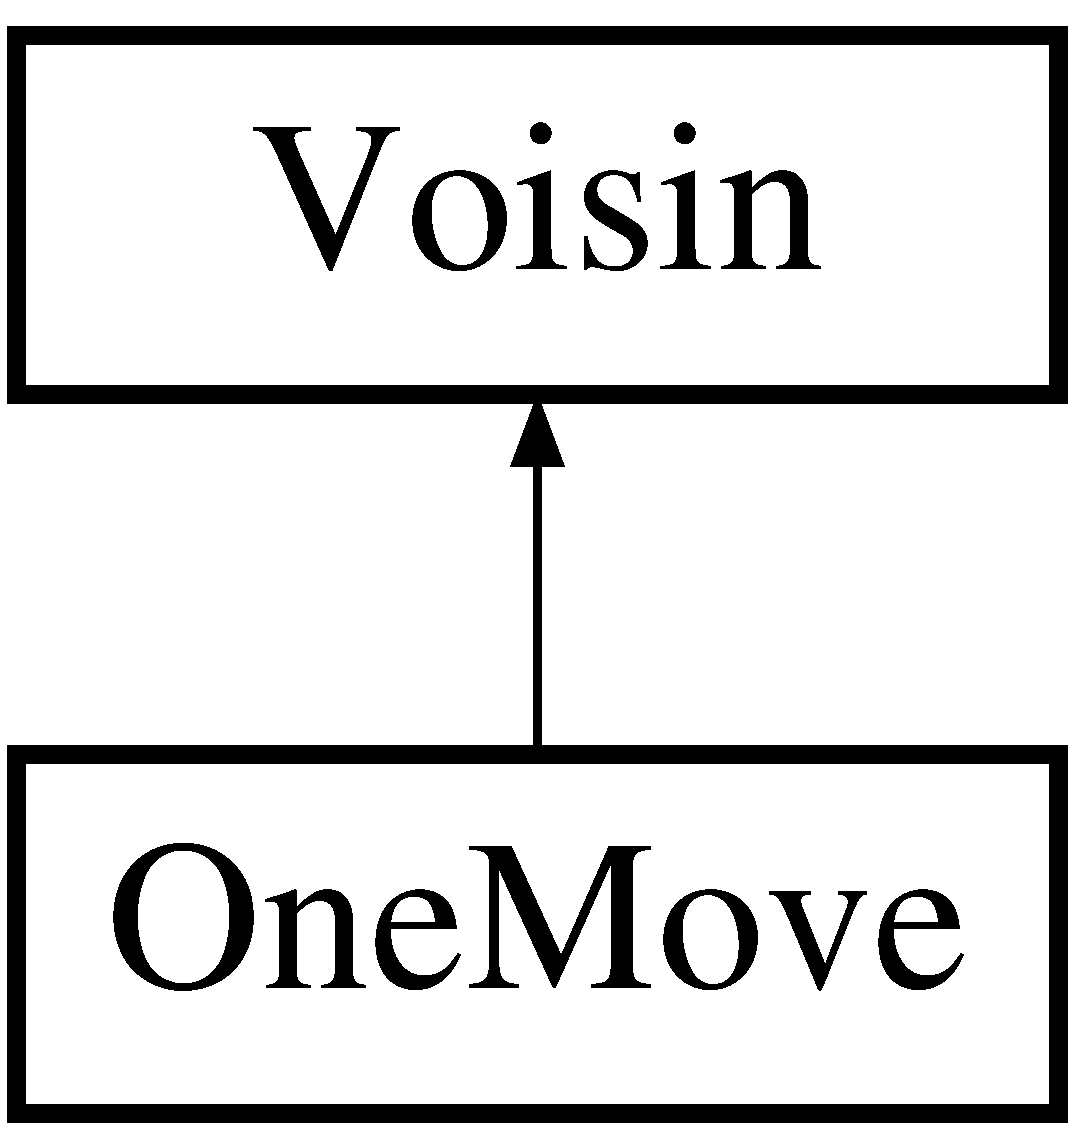
\includegraphics[height=2.000000cm]{classOneMove}
\end{center}
\end{figure}
\subsection*{Public Member Functions}
\begin{DoxyCompactItemize}
\item 
\hyperlink{classOneMove_a541f07108dca35fc6b352def2a040f26}{One\-Move} (int vertex, int ci, int cj)
\item 
int \hyperlink{classOneMove_a2fc5090fc05acec17a3ef1e30876e2b8}{get\-S} () const 
\item 
int \hyperlink{classOneMove_ad1224f9cdfb286dffee7a139a76a9642}{get\-Vki} () const 
\item 
int \hyperlink{classOneMove_a2b68813d5e5dd6bf3dd6d60bbb3ae5c5}{get\-Vkj} () const 
\item 
std\-::ostream \& \hyperlink{classOneMove_a14bbd56811a5863154f037e18c2d12e0}{print} (std\-::ostream \&out)
\end{DoxyCompactItemize}
\subsection*{Additional Inherited Members}


\subsection{Detailed Description}
Cette classe représente le premier voisinage décrit dans l'article lié à ce programme. Sa signature est la suivante \-: \hyperlink{classOneMove}{One\-Move} om(s,i,j) où s est le sommet à déplacer de sa couleur courante i vers la couleur j. 

\subsection{Constructor \& Destructor Documentation}
\hypertarget{classOneMove_a541f07108dca35fc6b352def2a040f26}{\index{One\-Move@{One\-Move}!One\-Move@{One\-Move}}
\index{One\-Move@{One\-Move}!OneMove@{One\-Move}}
\subsubsection[{One\-Move}]{\setlength{\rightskip}{0pt plus 5cm}One\-Move\-::\-One\-Move (
\begin{DoxyParamCaption}
\item[{int}]{vertex, }
\item[{int}]{ci, }
\item[{int}]{cj}
\end{DoxyParamCaption}
)}}\label{classOneMove_a541f07108dca35fc6b352def2a040f26}
Constructeur unique 
\begin{DoxyParams}{Parameters}
{\em vertex} & sommet concerné \\
\hline
{\em ci} & couleur source \\
\hline
{\em cj} & couleur destination \\
\hline
\end{DoxyParams}


\subsection{Member Function Documentation}
\hypertarget{classOneMove_a2fc5090fc05acec17a3ef1e30876e2b8}{\index{One\-Move@{One\-Move}!get\-S@{get\-S}}
\index{get\-S@{get\-S}!OneMove@{One\-Move}}
\subsubsection[{get\-S}]{\setlength{\rightskip}{0pt plus 5cm}int One\-Move\-::get\-S (
\begin{DoxyParamCaption}
{}
\end{DoxyParamCaption}
) const\hspace{0.3cm}{\ttfamily [inline]}}}\label{classOneMove_a2fc5090fc05acec17a3ef1e30876e2b8}
Getter sur le sommet \hypertarget{classOneMove_ad1224f9cdfb286dffee7a139a76a9642}{\index{One\-Move@{One\-Move}!get\-Vki@{get\-Vki}}
\index{get\-Vki@{get\-Vki}!OneMove@{One\-Move}}
\subsubsection[{get\-Vki}]{\setlength{\rightskip}{0pt plus 5cm}int One\-Move\-::get\-Vki (
\begin{DoxyParamCaption}
{}
\end{DoxyParamCaption}
) const\hspace{0.3cm}{\ttfamily [inline]}}}\label{classOneMove_ad1224f9cdfb286dffee7a139a76a9642}
Getter sur la couleur d'origine \hypertarget{classOneMove_a2b68813d5e5dd6bf3dd6d60bbb3ae5c5}{\index{One\-Move@{One\-Move}!get\-Vkj@{get\-Vkj}}
\index{get\-Vkj@{get\-Vkj}!OneMove@{One\-Move}}
\subsubsection[{get\-Vkj}]{\setlength{\rightskip}{0pt plus 5cm}int One\-Move\-::get\-Vkj (
\begin{DoxyParamCaption}
{}
\end{DoxyParamCaption}
) const\hspace{0.3cm}{\ttfamily [inline]}}}\label{classOneMove_a2b68813d5e5dd6bf3dd6d60bbb3ae5c5}
Getter sur la couleur d'arrivée \hypertarget{classOneMove_a14bbd56811a5863154f037e18c2d12e0}{\index{One\-Move@{One\-Move}!print@{print}}
\index{print@{print}!OneMove@{One\-Move}}
\subsubsection[{print}]{\setlength{\rightskip}{0pt plus 5cm}ostream \& One\-Move\-::print (
\begin{DoxyParamCaption}
\item[{std\-::ostream \&}]{out}
\end{DoxyParamCaption}
)\hspace{0.3cm}{\ttfamily [virtual]}}}\label{classOneMove_a14bbd56811a5863154f037e18c2d12e0}
Display 

Implements \hyperlink{classVoisin_a2ec06b60496a36a87abde5432198d7e6}{Voisin}.



The documentation for this class was generated from the following files\-:\begin{DoxyCompactItemize}
\item 
onemove.\-h\item 
onemove.\-cpp\end{DoxyCompactItemize}

\hypertarget{classSwap}{\section{Swap Class Reference}
\label{classSwap}\index{Swap@{Swap}}
}


{\ttfamily \#include $<$swap.\-h$>$}

Inheritance diagram for Swap\-:\begin{figure}[H]
\begin{center}
\leavevmode
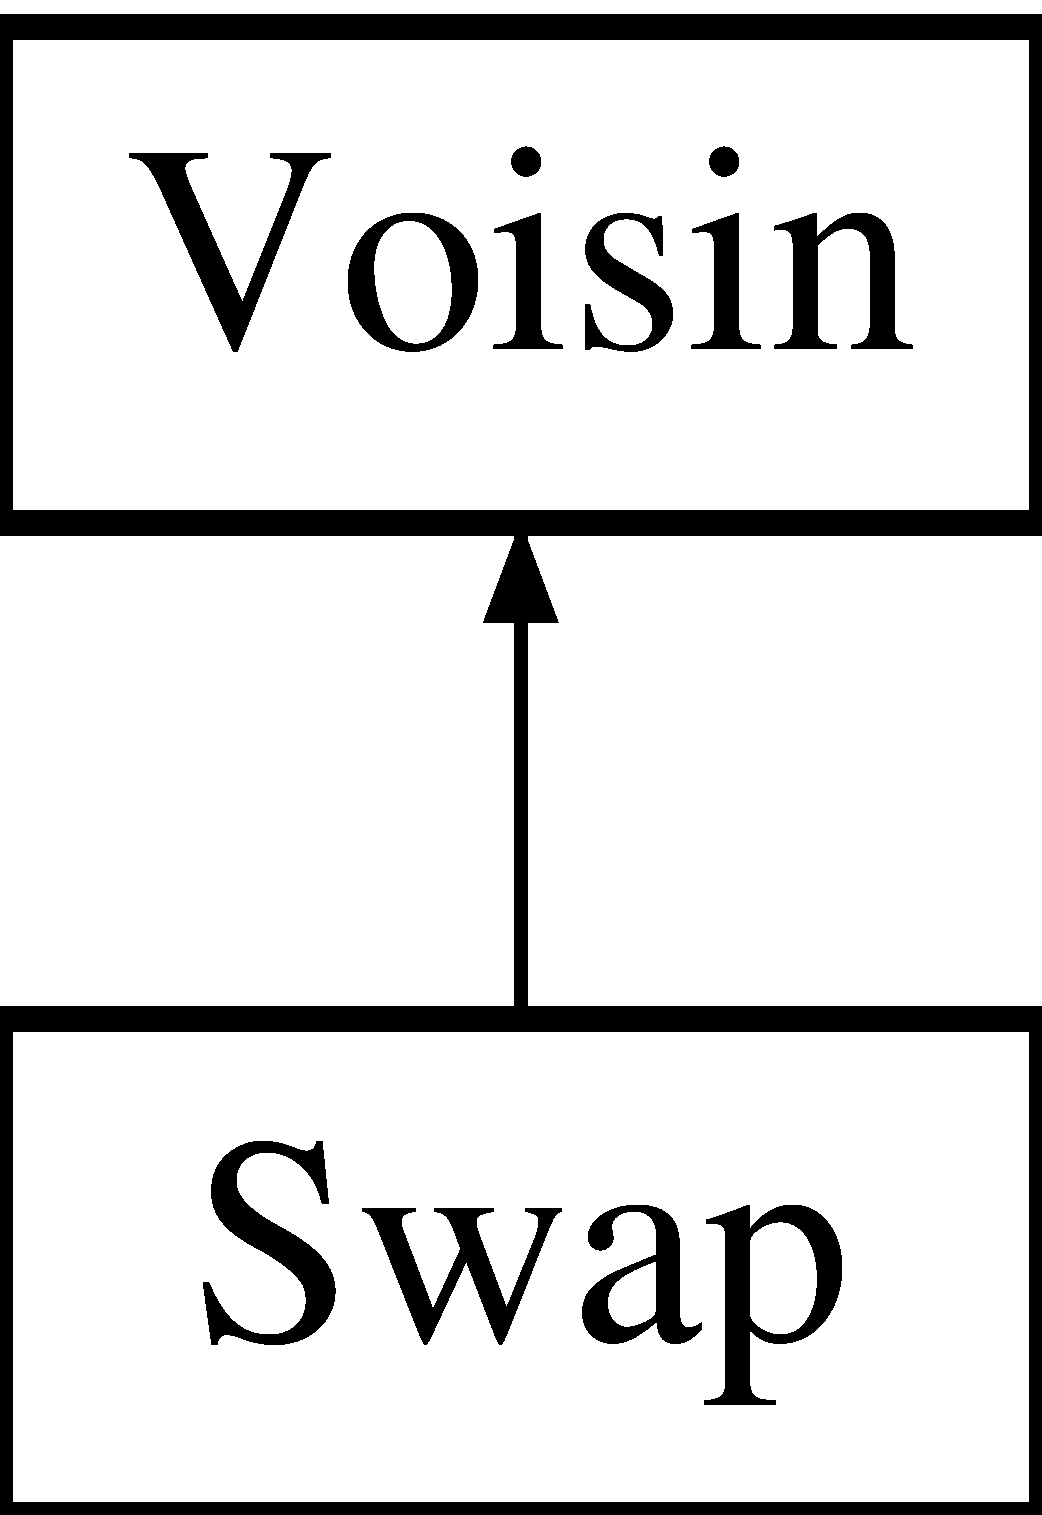
\includegraphics[height=2.000000cm]{classSwap}
\end{center}
\end{figure}
\subsection*{Public Member Functions}
\begin{DoxyCompactItemize}
\item 
\hyperlink{classSwap_a3afbc536a0c0ac95f29a93b9d318e2f0}{Swap} (int i, int j, int k, int l)
\item 
int \hyperlink{classSwap_a23dc26211a5fab2b455024ce063c0225}{get\-Si} () const 
\item 
int \hyperlink{classSwap_a58dbe1b75315cefde176ff15403715a9}{get\-Sj} () const 
\item 
int \hyperlink{classSwap_ade5279a41cf97b84e0582054ef8f8939}{get\-Ki} () const 
\item 
int \hyperlink{classSwap_a2cc551096dde6d0d437b4f0db618b3be}{get\-Kj} () const 
\item 
std\-::ostream \& \hyperlink{classSwap_af848d621402c8f39727adad5e0bff368}{print} (std\-::ostream \&out)
\end{DoxyCompactItemize}
\subsection*{Additional Inherited Members}


\subsection{Detailed Description}
Cette classe implément le second voisinage décrit dans l'article lié à ce programme. Sa signature est la suivante \-: \hyperlink{classSwap}{Swap} s(i,j,k,l) où i est coloré en k, j est coloré en l et le mouvement correspond à déplacer i vers la couleur l et le sommet j vers la couleur k. 

\subsection{Constructor \& Destructor Documentation}
\hypertarget{classSwap_a3afbc536a0c0ac95f29a93b9d318e2f0}{\index{Swap@{Swap}!Swap@{Swap}}
\index{Swap@{Swap}!Swap@{Swap}}
\subsubsection[{Swap}]{\setlength{\rightskip}{0pt plus 5cm}Swap\-::\-Swap (
\begin{DoxyParamCaption}
\item[{int}]{i, }
\item[{int}]{j, }
\item[{int}]{k, }
\item[{int}]{l}
\end{DoxyParamCaption}
)}}\label{classSwap_a3afbc536a0c0ac95f29a93b9d318e2f0}
Constructeur 
\begin{DoxyParams}{Parameters}
{\em i} & sommet Si \\
\hline
{\em j} & sommet Sj \\
\hline
{\em k} & couleur du sommet Si \\
\hline
{\em l} & couleur du sommet Sj \\
\hline
\end{DoxyParams}


\subsection{Member Function Documentation}
\hypertarget{classSwap_ade5279a41cf97b84e0582054ef8f8939}{\index{Swap@{Swap}!get\-Ki@{get\-Ki}}
\index{get\-Ki@{get\-Ki}!Swap@{Swap}}
\subsubsection[{get\-Ki}]{\setlength{\rightskip}{0pt plus 5cm}int Swap\-::get\-Ki (
\begin{DoxyParamCaption}
{}
\end{DoxyParamCaption}
) const\hspace{0.3cm}{\ttfamily [inline]}}}\label{classSwap_ade5279a41cf97b84e0582054ef8f8939}
Getter sur Ki \hypertarget{classSwap_a2cc551096dde6d0d437b4f0db618b3be}{\index{Swap@{Swap}!get\-Kj@{get\-Kj}}
\index{get\-Kj@{get\-Kj}!Swap@{Swap}}
\subsubsection[{get\-Kj}]{\setlength{\rightskip}{0pt plus 5cm}int Swap\-::get\-Kj (
\begin{DoxyParamCaption}
{}
\end{DoxyParamCaption}
) const\hspace{0.3cm}{\ttfamily [inline]}}}\label{classSwap_a2cc551096dde6d0d437b4f0db618b3be}
Getter sur Kj \hypertarget{classSwap_a23dc26211a5fab2b455024ce063c0225}{\index{Swap@{Swap}!get\-Si@{get\-Si}}
\index{get\-Si@{get\-Si}!Swap@{Swap}}
\subsubsection[{get\-Si}]{\setlength{\rightskip}{0pt plus 5cm}int Swap\-::get\-Si (
\begin{DoxyParamCaption}
{}
\end{DoxyParamCaption}
) const\hspace{0.3cm}{\ttfamily [inline]}}}\label{classSwap_a23dc26211a5fab2b455024ce063c0225}
Getter sur Si \hypertarget{classSwap_a58dbe1b75315cefde176ff15403715a9}{\index{Swap@{Swap}!get\-Sj@{get\-Sj}}
\index{get\-Sj@{get\-Sj}!Swap@{Swap}}
\subsubsection[{get\-Sj}]{\setlength{\rightskip}{0pt plus 5cm}int Swap\-::get\-Sj (
\begin{DoxyParamCaption}
{}
\end{DoxyParamCaption}
) const\hspace{0.3cm}{\ttfamily [inline]}}}\label{classSwap_a58dbe1b75315cefde176ff15403715a9}
Getter sur Sj \hypertarget{classSwap_af848d621402c8f39727adad5e0bff368}{\index{Swap@{Swap}!print@{print}}
\index{print@{print}!Swap@{Swap}}
\subsubsection[{print}]{\setlength{\rightskip}{0pt plus 5cm}ostream \& Swap\-::print (
\begin{DoxyParamCaption}
\item[{std\-::ostream \&}]{out}
\end{DoxyParamCaption}
)\hspace{0.3cm}{\ttfamily [virtual]}}}\label{classSwap_af848d621402c8f39727adad5e0bff368}
Display 

Implements \hyperlink{classVoisin_a2ec06b60496a36a87abde5432198d7e6}{Voisin}.



The documentation for this class was generated from the following files\-:\begin{DoxyCompactItemize}
\item 
swap.\-h\item 
swap.\-cpp\end{DoxyCompactItemize}

\hypertarget{classVoisin}{\section{Voisin Class Reference}
\label{classVoisin}\index{Voisin@{Voisin}}
}


{\ttfamily \#include $<$voisin.\-h$>$}

Inheritance diagram for Voisin\-:\begin{figure}[H]
\begin{center}
\leavevmode
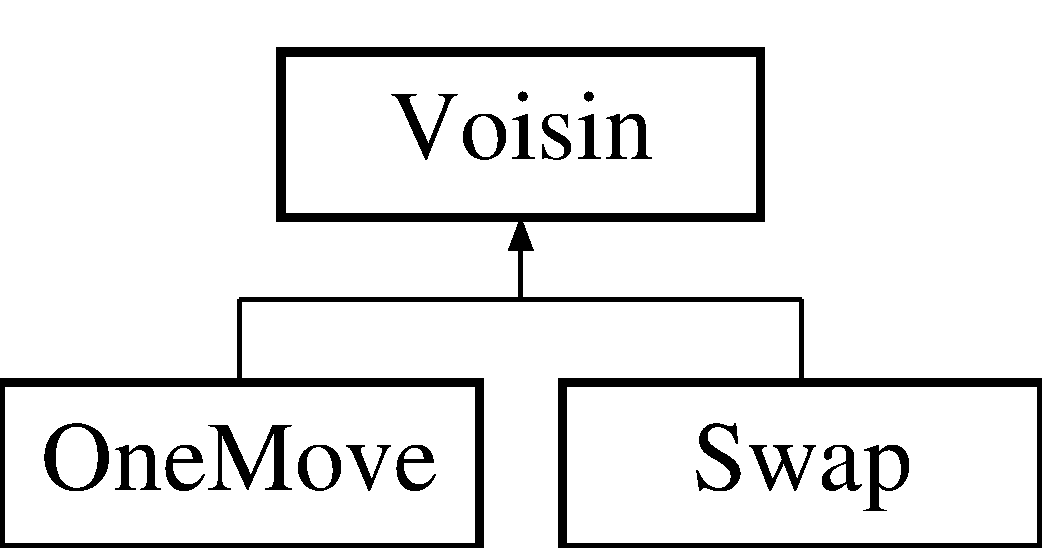
\includegraphics[height=2.000000cm]{classVoisin}
\end{center}
\end{figure}
\subsection*{Public Member Functions}
\begin{DoxyCompactItemize}
\item 
\hyperlink{classVoisin_ac7ebea598b40b3accadf277ee76dcf8e}{Voisin} ()
\item 
virtual \hyperlink{classVoisin_a44c12c877bbdedd0244890d4f9e69529}{$\sim$\-Voisin} ()
\item 
int \hyperlink{classVoisin_a565600a9d71ffc9c69fa2aebf8e874d9}{get\-Gain} () const 
\item 
void \hyperlink{classVoisin_ad0de7a06e897b38400e3adc3d295c674}{set\-Gain} (int x)
\item 
virtual std\-::ostream \& \hyperlink{classVoisin_a2ec06b60496a36a87abde5432198d7e6}{print} (std\-::ostream \&out)=0
\end{DoxyCompactItemize}
\subsection*{Static Public Member Functions}
\begin{DoxyCompactItemize}
\item 
static bool \hyperlink{classVoisin_a99d4a6956774fbb451ed9a935c607de0}{compare\-Gain} (const \hyperlink{classVoisin}{Voisin} $\ast$a, const \hyperlink{classVoisin}{Voisin} $\ast$b)
\end{DoxyCompactItemize}
\subsection*{Protected Attributes}
\begin{DoxyCompactItemize}
\item 
\hypertarget{classVoisin_ad2fe6936726b6a8e28c02bc07c7ce9a2}{int {\bfseries gain}}\label{classVoisin_ad2fe6936726b6a8e28c02bc07c7ce9a2}

\end{DoxyCompactItemize}
\subsection*{Friends}
\begin{DoxyCompactItemize}
\item 
std\-::ostream \& \hyperlink{classVoisin_a1840c108a788ffda111def8761fdac04}{operator$<$$<$} (std\-::ostream \&out, \hyperlink{classVoisin}{Voisin} \&v)
\end{DoxyCompactItemize}


\subsection{Detailed Description}
Cette classe représente la notion de voisin et du gain associé à celui ci. Un voisin étant défini par rapport à un problème donné, cette classe n'implémente que le gain, le reste devant être défini dans des sous-\/classes. 

\subsection{Constructor \& Destructor Documentation}
\hypertarget{classVoisin_ac7ebea598b40b3accadf277ee76dcf8e}{\index{Voisin@{Voisin}!Voisin@{Voisin}}
\index{Voisin@{Voisin}!Voisin@{Voisin}}
\subsubsection[{Voisin}]{\setlength{\rightskip}{0pt plus 5cm}Voisin\-::\-Voisin (
\begin{DoxyParamCaption}
{}
\end{DoxyParamCaption}
)}}\label{classVoisin_ac7ebea598b40b3accadf277ee76dcf8e}
Constructeur par défaut. \hypertarget{classVoisin_a44c12c877bbdedd0244890d4f9e69529}{\index{Voisin@{Voisin}!$\sim$\-Voisin@{$\sim$\-Voisin}}
\index{$\sim$\-Voisin@{$\sim$\-Voisin}!Voisin@{Voisin}}
\subsubsection[{$\sim$\-Voisin}]{\setlength{\rightskip}{0pt plus 5cm}virtual Voisin\-::$\sim$\-Voisin (
\begin{DoxyParamCaption}
{}
\end{DoxyParamCaption}
)\hspace{0.3cm}{\ttfamily [inline]}, {\ttfamily [virtual]}}}\label{classVoisin_a44c12c877bbdedd0244890d4f9e69529}
Destructeur virtuel 

\subsection{Member Function Documentation}
\hypertarget{classVoisin_a99d4a6956774fbb451ed9a935c607de0}{\index{Voisin@{Voisin}!compare\-Gain@{compare\-Gain}}
\index{compare\-Gain@{compare\-Gain}!Voisin@{Voisin}}
\subsubsection[{compare\-Gain}]{\setlength{\rightskip}{0pt plus 5cm}static bool Voisin\-::compare\-Gain (
\begin{DoxyParamCaption}
\item[{const {\bf Voisin} $\ast$}]{a, }
\item[{const {\bf Voisin} $\ast$}]{b}
\end{DoxyParamCaption}
)\hspace{0.3cm}{\ttfamily [inline]}, {\ttfamily [static]}}}\label{classVoisin_a99d4a6956774fbb451ed9a935c607de0}
Méthode de comparaison pour tri par ordre croissant de gain \hypertarget{classVoisin_a565600a9d71ffc9c69fa2aebf8e874d9}{\index{Voisin@{Voisin}!get\-Gain@{get\-Gain}}
\index{get\-Gain@{get\-Gain}!Voisin@{Voisin}}
\subsubsection[{get\-Gain}]{\setlength{\rightskip}{0pt plus 5cm}int Voisin\-::get\-Gain (
\begin{DoxyParamCaption}
{}
\end{DoxyParamCaption}
) const\hspace{0.3cm}{\ttfamily [inline]}}}\label{classVoisin_a565600a9d71ffc9c69fa2aebf8e874d9}
Getter sur le gain \begin{DoxyReturn}{Returns}
gain associé au voisin 
\end{DoxyReturn}
\hypertarget{classVoisin_a2ec06b60496a36a87abde5432198d7e6}{\index{Voisin@{Voisin}!print@{print}}
\index{print@{print}!Voisin@{Voisin}}
\subsubsection[{print}]{\setlength{\rightskip}{0pt plus 5cm}virtual std\-::ostream\& Voisin\-::print (
\begin{DoxyParamCaption}
\item[{std\-::ostream \&}]{out}
\end{DoxyParamCaption}
)\hspace{0.3cm}{\ttfamily [pure virtual]}}}\label{classVoisin_a2ec06b60496a36a87abde5432198d7e6}
Display 

Implemented in \hyperlink{classSwap_af848d621402c8f39727adad5e0bff368}{Swap}, and \hyperlink{classOneMove_a14bbd56811a5863154f037e18c2d12e0}{One\-Move}.

\hypertarget{classVoisin_ad0de7a06e897b38400e3adc3d295c674}{\index{Voisin@{Voisin}!set\-Gain@{set\-Gain}}
\index{set\-Gain@{set\-Gain}!Voisin@{Voisin}}
\subsubsection[{set\-Gain}]{\setlength{\rightskip}{0pt plus 5cm}void Voisin\-::set\-Gain (
\begin{DoxyParamCaption}
\item[{int}]{x}
\end{DoxyParamCaption}
)\hspace{0.3cm}{\ttfamily [inline]}}}\label{classVoisin_ad0de7a06e897b38400e3adc3d295c674}
Setter sur le gain 
\begin{DoxyParams}{Parameters}
{\em x} & valeur du gain \\
\hline
\end{DoxyParams}


\subsection{Friends And Related Function Documentation}
\hypertarget{classVoisin_a1840c108a788ffda111def8761fdac04}{\index{Voisin@{Voisin}!operator$<$$<$@{operator$<$$<$}}
\index{operator$<$$<$@{operator$<$$<$}!Voisin@{Voisin}}
\subsubsection[{operator$<$$<$}]{\setlength{\rightskip}{0pt plus 5cm}std\-::ostream\& operator$<$$<$ (
\begin{DoxyParamCaption}
\item[{std\-::ostream \&}]{out, }
\item[{{\bf Voisin} \&}]{v}
\end{DoxyParamCaption}
)\hspace{0.3cm}{\ttfamily [friend]}}}\label{classVoisin_a1840c108a788ffda111def8761fdac04}
Display 

The documentation for this class was generated from the following files\-:\begin{DoxyCompactItemize}
\item 
voisin.\-h\item 
voisin.\-cpp\end{DoxyCompactItemize}

%--- End generated contents ---

% Index
\newpage
\phantomsection
\addcontentsline{toc}{chapter}{Index}
\printindex

\end{document}
